
\documentclass[a4paper,UKenglish,cleveref, autoref, thm-restate,anonymous]{lipics-v2021}
%This is a template for producing LIPIcs articles. 
%See lipics-v2021-authors-guidelines.pdf for further information.
%for A4 paper format use option "a4paper", for US-letter use option "letterpaper"
%for british hyphenation rules use option "UKenglish", for american hyphenation rules use option "USenglish"
%for section-numbered lemmas etc., use "numberwithinsect"
%for enabling cleveref support, use "cleveref"
%for enabling autoref support, use "autoref"
%for anonymousing the authors (e.g. for double-blind review), add "anonymous"
%for enabling thm-restate support, use "thm-restate"
%for enabling a two-column layout for the author/affilation part (only applicable for > 6 authors), use "authorcolumns"
%for producing a PDF according the PDF/A standard, add "pdfa"

%\pdfoutput=1 %uncomment to ensure pdflatex processing (mandatatory e.g. to submit to arXiv)
%\hideLIPIcs  %uncomment to remove references to LIPIcs series (logo, DOI, ...), e.g. when preparing a pre-final version to be uploaded to arXiv or another public repository

%\graphicspath{{./graphics/}}%helpful if your graphic files are in another directory

\bibliographystyle{plainurl}% the mandatory bibstyle

% fast and exact
\title{Combining Predicted and Live Traffic with Time-Dependent A* Potentials}

%\titlerunning{Dummy short title} %TODO optional, please use if title is longer than one line

% \author{Jane {Open Access}}{Dummy University Computing Laboratory, [optional: Address], Country \and My second affiliation, Country \and \url{http://www.myhomepage.edu} }{johnqpublic@dummyuni.org}{https://orcid.org/0000-0002-1825-0097}{(Optional) author-specific funding acknowledgements}%TODO mandatory, please use full name; only 1 author per \author macro; first two parameters are mandatory, other parameters can be empty. Please provide at least the name of the affiliation and the country. The full address is optional. Use additional curly braces to indicate the correct name splitting when the last name consists of multiple name parts.

\author{Nils Werner}{Karlsruhe Institute of Technology, Germany}{}{}{}
\author{Tim Zeitz}{Karlsruhe Institute of Technology, Germany}{tim.zeitz@kit.edu}{https://orcid.org/0000-0003-4746-3582}{}

\authorrunning{N. Werner and T. Zeitz} %TODO mandatory. First: Use abbreviated first/middle names. Second (only in severe cases): Use first author plus 'et al.'

\Copyright{Nils Werner and Tim Zeitz} %TODO mandatory, please use full first names. LIPIcs license is "CC-BY";  http://creativecommons.org/licenses/by/3.0/

% \ccsdesc[100]{\textcolor{red}{Replace ccsdesc macro with valid one}} %TODO mandatory: Please choose ACM 2012 classifications from https://dl.acm.org/ccs/ccs_flat.cfm
\ccsdesc[500]{Theory of computation~Shortest paths}
\ccsdesc[300]{Mathematics of computing~Graph algorithms}
\ccsdesc[500]{Applied computing~Transportation}

\keywords{realistic road networks, shortest paths, live traffic, time-dependent routing} %TODO mandatory; please add comma-separated list of keywords

% \category{} %optional, e.g. invited paper

% \relatedversion{} %optional, e.g. full version hosted on arXiv, HAL, or other respository/website
%\relatedversiondetails[linktext={opt. text shown instead of the URL}, cite=DBLP:books/mk/GrayR93]{Classification (e.g. Full Version, Extended Version, Previous Version}{URL to related version} %linktext and cite are optional

%\supplement{}%optional, e.g. related research data, source code, ... hosted on a repository like zenodo, figshare, GitHub, ...
%\supplementdetails[linktext={opt. text shown instead of the URL}, cite=DBLP:books/mk/GrayR93, subcategory={Description, Subcategory}, swhid={Software Heritage Identifier}]{General Classification (e.g. Software, Dataset, Model, ...)}{URL to related version} %linktext, cite, and subcategory are optional

%\funding{(Optional) general funding statement \dots}%optional, to capture a funding statement, which applies to all authors. Please enter author specific funding statements as fifth argument of the \author macro.

\acknowledgements{I want to thank \dots}%optional

%\nolinenumbers %uncomment to disable line numbering



%Editor-only macros:: begin (do not touch as author)%%%%%%%%%%%%%%%%%%%%%%%%%%%%%%%%%%
\EventEditors{John Q. Open and Joan R. Access}
\EventNoEds{2}
\EventLongTitle{42nd Conference on Very Important Topics (CVIT 2016)}
\EventShortTitle{CVIT 2016}
\EventAcronym{CVIT}
\EventYear{2016}
\EventDate{December 24--27, 2016}
\EventLocation{Little Whinging, United Kingdom}
\EventLogo{}
\SeriesVolume{42}
\ArticleNo{23}
%%%%%%%%%%%%%%%%%%%%%%%%%%%%%%%%%%%%%%%%%%%%%%%%%%%%%%

\newcommand*{\pred}{p}
\newcommand*{\comb}{c}
\newcommand*{\opttt}{\mathcal{T}}
\newcommand*{\dist}{\mathcal{D}}
\newcommand*{\lb}{\mathcal{L}}

\newcommand*{\tdep}{\tau^{\operatorname{dep}}}
\newcommand*{\tmax}{\tau^{\max}}

\newcommand*{\gchu}{G^{\uparrow}}
\newcommand*{\gchd}{\overleftarrow{G^{\downarrow}}}
\newcommand*{\echu}{E^{\uparrow}}
\newcommand*{\echd}{\overleftarrow{E^{\downarrow}}}

\newcommand*{\pcfn}{\underline{b'^+}}
\newcommand*{\bucketlen}{x}

\usepackage[algo2e,vlined]{algorithm2e}
\usepackage{booktabs}

\begin{document}

\maketitle

%TODO mandatory: add short abstract of the document
\begin{abstract}
We study efficient and exact shortest path algorithms for routing on road networks with realistic traffic data.
For navigation applications, both predictions of future traffic flows and current traffic events play an important role in routing.
% In this work, we propose a combined model which integrates both aspects.
While preprocessing-based speedup techniques have been employed successfully to both settings individually, supporting a combined model poses significant challenges.
Supporting predicted traffic typically requires expensive and complex preprocessing while live traffic requires fast updates for regular adjustments.
We propose an A*-based solution to this problem.
To enable fast queries, we generalize A* potentials to time-dependency, i.e.\ estimates of the remaining distance also depended on the time a vertex is visited.
We then present, implement and evaluate two realizations of time-dependent potentials.
% propose td pots for better estimates and better usage of preprocessing to achieve faster TD queries than previously possible with A*
% becasue pots need not be exact higher flexibility to support live traffic
An experimental evaluation confirms the applicability of our potentials.
Live traffic updates can be realized within a fraction of a minute.
Queries can be answered two orders of magnitude faster than with Dijkstra's algorithm achieving almost real-time performance.
\end{abstract}

\section{Introduction}

An important feature of modern routing applications and navigation devices is the integration of traffic information into routing decisions.
The more comprehensive the considered traffic information, the better the suggested routes, the more accurate the predicted arrival times and ultimately, the more satisfied the users.
For routing, we can distinguish between two aspects of traffic:
On the one hand, there are \emph{predictable} traffic flows.
For example certain highways will consistently have traffic jams on weekday afternoons due to commuters driving home.
On the other hand, unexpected events such as accidents may also have significant influence on the \emph{current} traffic situation.
While it may be sufficient to focus on the current traffic situation to answer short-range routing request, mid- and long-range queries require taking both types of traffic into account.
% example with traffic jam now and in 300km?
We therefore aim to provide routing algorithms which incorporate \emph{combined} predicted and live traffic information.

A common approach for routing in road networks is to model the network as a directed graph where intersections become vertices and road segments become edges.
With edge weights representing travel times, routing requests can be answered by solving the classical shortest path problem.
When considering predicted traffic, edge weights can be modeled as functions of the daytime, which is commonly referred to as \emph{time-dependent routing}.
Dijkstra's algorithm can be used to solve these problems exactly and, at least from a theoretical perspective, efficiently~\cite{d-ntpcg-59}.
However, on the continental-sized road networks used in modern routing applications, it may take seconds to answer mid- or long-range queries which is too slow for most practical applications.
We therefore study algorithms to compute shortest paths significantly faster than Dijkstra's algorithm while retaining exactness.

In this work, we utilize the A* algorithm~\cite{hnr-afbhd-68} for this.
A* can be seen as an extension of Dijkstra's algorithm.
Dijkstra's algorithm explores all vertices closer to the origin than the destination by utilizing a queue where vertices are ordered by their distance from the origin vertex.
A* changes the order in which vertices are visited by adding an estimate of the remaining distance to the queue key, sometimes called \emph{heuristic} or \emph{potential}.
The performance depends on the tightness of these estimates.
The algorithmic core idea of this work are time-dependent potential functions, i.e.\ we obtain tighter estimates and therefore faster queries by taking the time a vertex is visited into account.

\subsection{Related Work}

Efficient and exact route planning in road networks has received a significant amount of research effort in the past decade.
Since a comprehensive overview is beyond the scope of this paper, we refer to~\cite{bdgmpsww-rptn-16} for an overview.
An approach that has proven quite effective is to exploit that road networks rarely change and usually many queries have to be answered on the same network.
Thus, these queries can be accelerated by computing auxiliary data in an off-line preprocessing phase.

A popular technique following this approach is \emph{Contraction Hierarchies} (CH)~\cite{gssv-erlrn-12}.
During the preprocessing vertices are heuristically ranked by importance (more important vertices are part of more shortest paths).
Shortcut edges are inserted to skip over unimportant vertices.
This allows for a very fast query where only few vertices are explored.
On typical continental-sized benchmark instances, queries take well below a millisecond.
\emph{Multi-Level Dijkstra} (MLD)~\cite{swz-umlgt-02} is a similar approach which also utilizes shortcut edges but inserts them based on a multi-level partitioning.
It achieves slightly slower query times around a millisecond.
MLD is popular for being the first algorithm to support the concept of \emph{customizability} and therefore sometimes also referred by \emph{Customizable Route Planning} (CRP)~\cite{dgpw-crprn-13}.
The \emph{customization} is a second faster preprocessing phase which allows integrating arbitrary weight functions (or live traffic updates the current weights) into the auxiliary data without rerunning the whole slow first preprocessing phase.
The MLD customization takes a couple of seconds which allows running it every minute.
CH was later generalized to support customizability as well which resulted in Customizable Contraction Hierarchies (CCH)~\cite{dsw-cch-15}.

Both CH and MLD have been extended to time-dependent routing.
However, dealing with weight functions instead of scalar weights makes the preprocessing much harder and leads to difficult trade-offs.
TCH~\cite{bgsv-mtdtt-13} has fast queries but a very expensive preprocessing phase (may take hours) and may produce prohibitive amounts of auxiliary data (> 100\,GB).
% TODO 3-phase not introduced
TD-CRP~\cite{bdpw-dtdrp-16} (the MLD variant) still follows a 3-phase approach and has a relatively fast customization phase.
However, this is only possible by giving up exactness.
Also, TD-CRP does not support path unpacking.
CATCHUp~\cite{swz-sfert-21} adapts CCH to the time-dependent setting and has fast and exact queries with significantly reduced memory consumption.
While it has a customization phase, running it takes significantly longer than a traditional CCH or CRP customization.
On the benchmark graphs used in this paper, a CATCHUp customization may even take hours, which is too slow for a live traffic updates setting.
% TDS?, (Shark?)

A* has also been utilized in speed-up techniques for routing in road networks.
With ALT~\cite{gh-cspas-05,gw-cppsp-05}, a few landmark vertices are selected during preprocessing.
From and to these vertices, distances to all other vertices are precomputed.
During queries, these distances are combined with the triangle inequality to obtain distance estimates to the target vertex.
ALT has also received research interest in areas beyond route planning.
However, query times are significantly slower than with shortcut-based approaches such as CH or MLD.
ALT has also been extended to dynamic and time-dependent settings~\cite{dn-crdtd-12}. % combined?
However, the model studied there is not as general as with customization based approaches.
% Core-ALT?

Another more recent A*-based approach is CH-Potentials~\cite{strasser_et_al:LIPIcs.SEA.2021.6}.
CH-Potentials extract exact distances from a CH using Lazy RPHAST which we also heavily use in this work.
This leads to tighter estimates and faster queries than possible with ALT.
CH-Potentials can be applied to a variety of routing problem variants and the original publication even mentions a combination of live and predicted traffic.
However the reported query times are a above 100\,ms which we consider too slow for practical applications.

\subsection{Contribution}

In this work, we introduce a time-dependent generalization of A* potentials.
We present two simple extensions of Lazy RPHAST which realize a time-dependent potential function and discuss how to apply them to queries in a combined live and predicted traffic setting.
An extensive evaluation confirms the applicability of our algorithms.
Queries incorporating both predicted and the current traffic can be answered within few tenths of milliseconds.
Live traffic updates can be integrated within a fraction of a minute.
Our time-dependent potentials are up to an order of magnitude faster than the classical Lazy RPHAST-based CH-Potentials and about two orders of magnitude faster than Dijkstra's algorithm.
% Introduce A* with TDPot
% Introduce 2 TDPots
% Show how to apply them to live traffic
% Extensive eval
% up to one order of mag over time independent pot
% 2 orders of magnitude over dijkstra

\section{Preliminaries}
We consider simple directed graphs $G=(V,E)$ with $n=|V|$ vertices and $m=|E|$ edges.
We use $uv$ as a short notation for an edge from a \emph{tail} vertex $u$ to \emph{head} vertex $v$.
Weight functions $w : E \to (\mathbb{Z} \to \mathbb{Z}^{\geq 0})$ map edges to time-dependent functions which in turn map a departure $\tau$ at the tail $u$ to a travel time $w(uv)(\tau)$.
% The arrival at the head $v$ is thus $w(uv)(\tau) + \tau$.
To simplify notation we will often write $w(uv, \tau)$.
When it is clear from context that we talk about constant functions, we omit the time argument and write $w(uv)$.
The reversed graph $\overleftarrow{G} = (V, \overleftarrow{E})$ contains reversed edges $vu$ for every edge $uv \in E$ and $\overleftarrow{w}(vu) = w(uv)$ is the corresponding (time-independent) reversed weight function.
% We extend the weight function definition to paths:
The travel time of a path $P = (v_1,\dots,v_k)$ can be obtained by successively evaluating the edges travel times: $w(P, \tau) = w(v_1 v_2, \tau) + w((v_2,\dots,v_k), \tau + w(v_1 v_2, \tau))$.
We denote the travel time of the shortest path between vertices $s$ and $t$ as $\dist_w(s,t,\tdep)$.
We assume that all travel time functions adhere to the \emph{First-In First-Out} (FIFO) property, i.e.\ departing later may never lead to an earlier arrival.
Formally stated, this means $\tau + w(\tau) \leq \tau + \epsilon + w(\tau + \epsilon)$ for any $\epsilon \geq 0$.
% TODO explain waiting?
With non-FIFO travel time functions, the shortest path problem becomes \textsf{NP}-hard~\cite{or-tnp-89}.

\subsection{Problem Model}

% phases
We consider an application model with three phases.
During the \emph{preprocessing} phase, the graph $G=(V,E)$ and a weight function $\pred$ of time-dependent traffic predictions are given.
Predicted travel time functions are periodic piecewise linear functions represented by a sequence of breakpoints covering one day.
A preprocessing algorithm may now precompute auxiliary data which may take several hours.
Preprocessing should still be fast enough to rerun it on a daily basis.
In the \emph{update} phase, a weight function $l$ of currently observed (constant) live travel times are given for the current moment $\tau^{\operatorname{now}}$.
Further, each edge has a point in time $\tau^{\operatorname{end}}(e)$ when we switch back to the predicted travel time.
For edges without live traffic data, we set $\tau^{\operatorname{end}}(e) = \tau^{\operatorname{now}}$.
We assume that traffic predictions are conservative estimates and that live traffic will only be slower due to accidents and other traffic incidents.
Thus, we define the combined weight function as follows:
$\comb(e, \tau) = \max(\pred(e, \tau), \min(l(e), \pred(e, \tau^{\operatorname{end}}(e)) + \tau^{\operatorname{end}}(e) - \tau))$.
The update phase will be repeated frequently (every few minutes) and should therefore be as fast as possible.
% We do not call this phase \emph{customization} because we use customization algorithms from CCH and CATCHUp during both the preprocessing and the update phases.
During the final \emph{query} phase, many shortest path queries $(s,t,\tdep)$ where $\tdep \geq \tau^{\operatorname{now}}$ should be answered as quickly as possible by obtaining the path $P = (s,\dots,t)$ that minimizes $\comb(P, \tdep)$.
We discuss this traffic model further in Appendix~\ref{sec:appendix:model}.

\subsection{Fundamental Algorithms}

% distance vs arrival times
\emph{Dijkstra's algorithm} computes $\dist_w(s,t,\tdep)$ by exploring vertices ordered by increasing distance from $s$ until $t$ is reached.
The distances from $s$ of each vertex $u$ are tracked in an array $\mathtt{D}[u]$, initially set to $\infty$ for all vertices.
A priority queue with vertices ordered by their distance from $s$ is maintained.
The priority queue is initialized with $s$ and $\mathtt{D}[u]$ set to $\tdep$.
In each iteration, the next closest vertex $u$ is extracted from the queue and \emph{settled}.
Outgoing edges $uv$ are \emph{relaxed}, i.e.\ the algorithm checks if $\mathtt{D}[u] + w(uv, \mathtt{D}[u])$ improves $\mathtt{D}[v]$.
If so, the queue position of $v$ is adjusted accordingly.
Once $t$ was settled, the final distance is known and the search can terminate.
We denote the vertices visited during a query as \emph{search space}.

% heurisitc vs potential
A* is an extension of Dijkstra's algorithm where the search is guided towards the target through a potential function $\pi_t$ which maps vertices to an estimate of the remaining distance.
This estimate is added to the queue key.
Thus, vertices closer to the target a visited earlier and the search space becomes smaller.
%
In this work, we use a time-dependent generalization $\pi_t : V \to (T \to \mathbb{Z}^{\geq 0})$ of A* potentials, i.e.\ estimates are a function of the time.
This allows us to obtain tighter estimates and enables faster queries.
% Analogue to classical potentials, t
There are three important properties of time-dependent potentials to consider when arguing about the correctness of A*:
\begin{itemize}
  \item Lower bound: $\pi_t(v, \tau) \leq \dist(v,t,\tau)$ for all vertices $v \in V$ and times $\tau = \dist_w(s,v,\tdep)$.
  A* with a lower bound potential will have found the correct distance once the target vertex is settled.
  However, with only lower bound potentials, A* may settle vertices multiple times.
  In theory, this can lead to exponential running time.
  \item Feasibility: $w(uv, \tau) + \pi_t(v, \tau + w(uv, \tau)) - \pi_t(u, \tau) \geq 0$ for all edges $uv \in E$ and times $\tau > \dist_w(s,u,\tdep)$.
  A* is equivalent to Dijkstra's algorithm on a graph with modified weights.
  When feasibility holds, these modified weights are positive which implies correctness.
  When $\pi_t(t, \tau) = 0$, feasibility also implies the lower bound property.
  \item First-In First-Out (FIFO): $\pi_t(v, \tau) \leq \pi_t(v, \tau + \epsilon) + \epsilon$ for $v \in V$, $\tau > \dist_w(s,u,\tdep)$ and $\epsilon \geq 0$.
  It must always hold or worse distances might have better queue keys.
  % This property has no time-independent equivalent because it trivially holds in this case.
\end{itemize}
In Appendix~\ref{sec:appendix:correctness} we derive and discuss these correctness properties in detail and formally prove that queries will be answered correctly with these properties.
Note that these properties only need to hold for certain times $\tau$.
Our proposed potentials heavily rely on this and only compute data for the specific times necessary to answer a query correctly.

% \subsection{Contraction Hierarchies}

\emph{Contraction Hierarchies} (CH)~\cite{gssv-erlrn-12} is a speed-up technique to accelerate shortest path computations on time-independent road networks through precomputation.
% For a detailed discussion we refer to~\cite{gssv-erlrn-12}.
% Here, we briefly introduce necessary notation and concepts used in this paper.
During the preprocessing, a total order $v_1 < \dots < v_n$ among all vertices $v_i \in V$ by ``importance'' is determined heuristically, where more important vertices should lie on more shortest paths.
Intuitively, vertices on highways are more important than vertices on rural streets.
Then, an \emph{augmented graph} $G^+ = (V, E^+)$ with additional \emph{shortcut edges} and weights $w^+$ is constructed.
Shortcut edges $uv$ allow to ``skip over'' paths $(u,\dots,x_i,\dots,v)$ where $x_i < u \land x_i < v$.
Therefore, $w^+(uv)$ gets the length of the shortest such path.
We sometime refer to $G^+$ split into an upward graph $\gchu = (V, \echu)$ which contains only edges $uv$ where $v > u$ and a downward graph $G^{\downarrow} = (V, E^{\downarrow})$ vice versa.
The augmented graph has the property that between any two vertices $s$ and $t$ there exists a path $P$ with $w^+(P) = \dist_w(s,t)$ and $v \geq \min(s, t) \forall v \in P$.
Such a path can be found by running the bidirectional variant of Dijkstra's algorithm from $s$ on $\gchu$ and from $t$ on $\gchd$.
Because only few vertices are reachable in this \emph{CH search space}, queries are very fast.

In this work we build on \emph{Customizable Contraction Hierarchies} (CCH)~\cite{dsw-cch-15}.
For CCH, the construction of the augmented graph is split in two phases.
In the first phase, the topology of the augmented graph is constructed without considering any weight functions.
It therefore is valid for \emph{all} weight functions.
In the second phase, the \emph{customization}, the weights $w^+$ of the augmented graph are computed for a given weight function $w$.
The customization can be parallelized efficiently~\cite{bsw-rttau-19}.

% \subsection{Lazy RPHAST and CH-Potentials}

\begin{algorithm2e}
\KwData{$\mathtt{D}^{\downarrow}[u]$: tentative distance from $u$ to $t$ computed by Dijkstra's algorithm on $\gchd$}
\KwData{$\mathtt{D}[u]$: memoized final distance from $u$ to $t$, initially $\bot$}
\SetKwFunction{Dist}{ComputeAndMemoizeDist}
\SetKwProg{Fn}{Function}{:}{}
\Fn{\Dist{$u$}}{
    \If{$\mathtt{D}[u] = \bot$}{
        $\mathtt{D}[u]\leftarrow \mathtt{D}^{\downarrow}[u]$\;
        \For{all edges $uv \in \echu$}{
            $d \leftarrow \Dist(v)$\;
            \If{$d + w^+(uv) < \mathtt{D}[u]$}{
                $\mathtt{D}[u] \leftarrow d + w^+(uv)$\;
            }
        }
    }
    \Return{$\mathtt{D}[u]$}\;
}
\caption{Computing the distance from a single vertex $u$ to $t$ with Lazy RPHAST}
\label{algo:lazy_rphast}
\end{algorithm2e}

\emph{Lazy RPHAST}~\cite{strasser_et_al:LIPIcs.SEA.2021.6} is a (C)CH query variant to incrementally compute distances from many sources toward a common target.
The first step is a run Dijkstra's algorithm on $\gchd$ from $t$, similarly to a regular CH query.
The second Dijkstra search is replaced with a recursive depth-first search (DFS) which memoizes distances.
Algorithm~\ref{algo:lazy_rphast} depicts this routine which will be called for all sources.
If the distance of a vertex $u$ was previously computed, the routine terminates immediately and returns the memoized value $\mathtt{D}[u]$.
Otherwise, the distance for all upward neighbors $v$ is obtained recursively.
The final distance is the minimum over the paths distances $w^+(uv) + \mathtt{D}[v]$ through the upward neighbors and the distance possibly found in the backward search $\mathtt{D}^{\downarrow}[u]$.
Using a DFS to compute shortest distances works because $\gchu$ is a directed acyclic graph.
Using Lazy RPHAST as an A* potential is called \emph{(C)CH-Potentials}.
The authors of~\cite{strasser_et_al:LIPIcs.SEA.2021.6} describe additional optimizations for A* which we also utilize.
The goal is to reduce the impact of the potential evaluation overhead by avoiding unnecessary potential evaluations, for example for chains of degree-two vertices.

\section{Time-Dependent A* Potentials}

In this section, we propose two time-dependent A* Potentials which are both extensions of Lazy RPHAST.
Lazy RPHAST/CH-Potentials is already quite an efficient potential and obtains exact distances with respect to scalar lower bound weights, i.e.\ the tightest possible estimates with a time-independent potential definition.
To outperform CH-Potentials, we must not only obtain significantly tighter estimates but also be careful to not make the potential evaluation too expensive.
Therefore, we avoid costly operations on functions and work with scalar values as much as possible.
Also, even though our potentials are time-dependent, computed estimates during an individual query will typically \emph{not} change depending on the visit time.

\subsection{Multi-Metric Potential}

Let $(s,t,\tdep)$ be a query and $\tmax = \tdep + \dist_c(s,t,\tdep)$ the optimal arrival at the target.
Consider any $\tau' \leq \tdep$, $\tau'' \geq \tmax$ and the weight function $l_{[\tau', \tau'']}(e) = \min_{\tau' \leq \tau \leq \tau''}\pred(e, \tau)$. % where $\pred$ are the predicted travel times.
Clearly, $\dist_{l_{[\tau', \tau'']}}(v,t)$ provides lower bound estimates of distances to the target vertex during the time relevant for this query.
If $\tau'$ and $\tau''$ are close to $\tdep$ and $\tmax$ and if the difference between $\tau'$ and $\tau''$ is not too big, the estimates will be significantly tighter than global lower bound distances.
The \emph{Multi-Metric Potential} is based on this observation.
Instead of using a single potential based on a global lower bound valid for the entire time, we process multiple lower bound weight functions valid for different time intervals.
At query time, we then select an appropriate weight function.
Efficiently computing distances with respect to the selected weight function is done with the Lazy RPHAST.

\subparagraph{Phase Details.}
The very first step of the preprocessing for this potential is to perform the regular CCH preprocessing, i.e.\ compute an importance ordering and construct the unweighted augmented graph.
Now let $I$ be a set of time intervals.
In our implementation,
we cover the time between 6:00 and 22:00 with intervals of length one, two, four and eight hours, starting every 30 minutes,
and one interval covering the entire day.
We do not keep any additional intervals between 22:00 and 6:00 as most edges will have their freeflow travel time during this time.
Thus, the lower bound weights in these intervals would be equal to the full-day lower bounds.
During preprocessing, for each interval $[\tau_i', \tau_i''] \in I$, we extract lower bound functions $l_{[\tau_i', \tau_i'']}$ and run the CCH basic customization algorithm for each interval to obtain $l_{[\tau_i', \tau_i'']}^+$.
This can be trivially parallelized.
Also, the customization can be parallelized internally.
For further engineering details, we refer to~\cite{dsw-cch-15,bsw-rttau-19,ghuw-fbndocch-19}.

During the update phase, we compute an additional lower bound weight function for $[\tau^{\operatorname{now}}, \tau^{\operatorname{now}} + 59\,\operatorname{minutes}]$ which incorporates the current live traffic situation $\comb$ and run the basic customization for it.
Further, we extract an upper bound weight function $\comb_{\max}$ valid for the entire day with respect to both the predicted and the live traffic and perform the CCH basic customization to obtain $\comb^+_{\max}$.

The query starts with a classical CCH query on the customized upper bound $\comb^+_{\max}$ to obtain a pessimistic estimate of $\tmax$.
We then select the shortest interval $[\tau_i', \tau_i'']$ such that $[\tdep,\tmax] \subseteq [\tau_i', \tau_i'']$.
Running Lazy RPHAST on $G^*_l$ with the customized weight function $l_{[\tau_i', \tau_i'']}^+$ of this interval yields the desired potential function.
See Appendix~\ref{sec:appendix:optimizations} for some additional optimizations.

\subparagraph{Correctness.}
For any given single query, the multi metric potential actually is a time-independent potential which returns exact shortest distance with respect to a valid lower bound weight function.
Constant potentials trivially adhere to the strong FIFO property.
Also, as shown in~\cite{strasser_et_al:LIPIcs.SEA.2021.6}, shortest distances by a lower bound weight function are feasible.

\subsection{Interval-Minimum Potential}

The \emph{Interval-Minimum Potential} is a time-dependent adaptation of the Lazy RPHAST algorithm.
Where Lazy RPHAST has a single scalar (lower bound) weight for each edge, the Interval-Minimum Potential has a lower bound function.
This allows for tighter estimates but introduces new challenges.
First, we need an augmented graph with sufficiently accurate time-dependent lower bounds.
We utilize the existing CATCHUp customization~\cite{swz-sfert-21} because it is also based on CCH.
Second, storing the shortcut travel time functions $w^+$ can be very expensive in terms of memory consumption.
Also, the representation as a list of breakpoints makes the evaluation much more expensive than looking up a scalar weight.
We therefore resort to a different representation and store functions as piecewise constant values in buckets of equal duration.
In our implementation, we split the day into 96 buckets of length 15 minutes.
Third, evaluating these functions requires a time of evaluation.
While $\pi_t(v, \tau)$ includes the time argument $\tau$ for the time at $v$, Lazy RPHAST also needs a time for every recursive invocation.
We therefore apply Lazy RPHAST a second time on a global upper $\comb_{\max}^+$ and lower bound weight function $\pred_{\min}^+$ to obtain arrival intervals for arbitrary vertices.

\subparagraph{Phase Details.}
The first preprocessing step is the CCH preprocessing.
For the second step, we need to obtain time-dependent travel times for the augmented graph $G^+$ based on the predicted traffic weights $p$.
For this, we use CATCHUp~\cite{swz-sfert-21}, which is a time-dependent adaptation of CCH.
% TCH also possible
The CATCHUp customization yields for each edge in $uv \in E^+$ approximated \emph{time-dependent} lower bound functions $\underline{b^+}$.
We transform the time-dependent piecewise linear lower bound functions $\underline{b^+}$ into piecewise \emph{constant} lower bound functions
$\pcfn(uv, \tau) := \min_{\lfloor \frac{\tau}{\bucketlen} \rfloor \bucketlen \leq \tau' < (\lfloor \frac{\tau}{\bucketlen} \rfloor + 1) \bucketlen} \underline{b^+}(uv, \tau')$
where $\bucketlen$ is the length of each constant segment, i.e.\ in our case 15 minutes.
This enables a compact representation because functions can be represented with a fixed number of values per edge.
We additionally derive a scalar lower bound $b^+_{\min}$.
Note that $b^+_{\min}$ is typically much tighter than bounds obtained by a time-independent customization on input function bounds, i.e.\ $w^+_{\min}$.

For the update phase we extract an upper bound weight function $\comb_{\max}$ for the entire day valid with respect to both the predicted and the live traffic.
Then we run the CCH customization algorithm to obtain $\comb^+_{\max}$.

% make sure its clear that the lazy rphast remains time-independent
The query consists of two instantiations of the Lazy RPHAST algorithm.
The first one uses the scalar bounds $b^+_{\min}$ and $\comb^+_{\max}$ and computes arrival intervals at arbitrary vertices.
Since arrival intervals are distances from the source vertex, we have to Lazy RPHAST in reverse direction, i.e.\ first, we run Dijkstra's algorithm from $s$ on $\gchu$ and then, we apply the recursive distance-memoizing DFS on $\gchd$ for any vertex for which we want to obtain an arrival interval.
With these arrival intervals, we can now compute lower bounds to the target with the second Lazy RPHAST instantiation, which uses the time-dependent lower bounds $\pcfn$.
The first step is to run Dijkstra's algorithm from $t$ on $\gchd$.
To relax an edge $uv \in \echd$, we first need to obtain an arrival interval $[\tau_{\min}, \tau_{\max}]$ at $v$ using Lazy RPHAST on the bounds.
This allows us to determine a tight lower bound for $vu$ the relevant time and we can then check if we can improve the lower bound from $v$ to $t$, i.e.\
$\mathtt{D}^{\downarrow}[v] \leftarrow \min(\mathtt{D}^{\downarrow}[v], \mathtt{D}^{\downarrow}[u] + \min_{\tau \in [\tau_{\min}, \tau_{\max}]} \pcfn(vu, \tau))$.
Having established preliminary backward distances for all vertices in the CH search space of $t$, we can now compute estimates with the recursive distance-memoizing DFS.
To obtain a distance estimate for vertex $u$, we first recursively compute distance estimates $\mathtt{D}^{\downarrow}[v]$ for all upward neighbors $v$ where $uv \in \echu$.
Then, we use Lazy RPHAST on the bounds to obtain an arrival interval at $[\tau_{\min}, \tau_{\max}]$ at $u$.
Finally, we relax the upward edges $uv$ set $\mathtt{D}^{\downarrow}[u] \leftarrow \min(\mathtt{D}^{\downarrow}[u], \mathtt{D}^{\downarrow}[v] + \min_{\tau \in [\tau_{\min}, \tau_{\max}]} \pcfn(uv, \tau))$.
This yields the final estimate for $u$.

Choosing the right memory layout for the bucket weights is crucial for the performance.
We do store all edge weights of each bucket consecutively.
Typically, only few buckets per edge are relevant, because the arrival intervals are relatively tight.
Also, all outgoing edges of each vertex are evaluated consecutively.
Thus, having their weights for the same bucket close to each other increases cache hits.
See Appendix~\ref{sec:appendix:optimizations} for additional optimizations.

\subparagraph{Correctness.}
The Interval-Minimum Potential is not feasible because we use piecewise constant functions for the the shortcut travel time lower bounds.
Still, it does satisfy the strong FIFO property because for any given single query, the estimates are constant.
Moreover, the estimates are lower bounds on the distances.
This directly follows from the correctness of the CATCHUp preprocessing and the Lazy RPHAST algorithm.

\subsection{Compression}\label{sec:compression}

Both our time-dependent potentials have to store a significant number of weight functions.
This can lead to problematic memory consumption.
However, since we only need lower bounds, we can merge lower bound weight functions into a combined weight function with the respective minimum weights.
Thus, by trading some tightness, we can reduce memory consumption.
Both potentials can handle merged lower bound functions with a layer of indirection which maps each bucket or interval to a weight function id.
When merging to weight functions, we let both buckets/intervals point to the same weight function id.

We now discuss an efficient and well parallelizable algorithm to iteratively merge weight functions until only $k$ functions remain.
In each step, we merge the pair of weight functions with the minimal sum of squared differences over all edge weights.
Since comparing all pairs of weight functions is expensive, we track the minimum difference sum $\delta_{\min}$ we have found so far and stop any comparison where the sum exceeds $\delta_{\min}$.
However, even when stopping a comparison, we store the preliminary sum and the edge id up to which we have summed up the differences.
Then, we do not need to start from scratch should we need to continue to compare this particular pair of weight functions.
Finally, we maintain all pairs of weights along with the (possibly preliminary) difference sums in a priority queue ordered by the difference sums.
When merging two weight functions, all other associated queue entries are removed from the queue and new entries for comparisons between the new weight function and all other functions are inserted.
To determine the next weight function pair to merge, unfinished weight function pairs are popped from the queue and processed in parallel.
The minimum difference is tracked in an atomic variable.

\section{Evaluation}
% env
\subparagraph{Environment} Our benchmark machine runs openSUSE Leap 15.3 (kernel 5.3.18), and has 192\,GiB of DDR4-2666 RAM and two Intel Xeon Gold 6144 CPUs, each of which has eight cores clocked at 3.5\,GHz and 8~$\times$~64\,KiB of L1, 8~$\times$~1\,MiB of L2, and 24.75\,MiB of shared L3 cache.
Hyperthreading was disabled and parallel experiments use 16 threads.
We implement our algorithms in Rust\footnote{The code for this paper and all experiments is available at \url{https://github.com/kit-algo/tdpot}} and compile them with \texttt{rustc 1.61.0-nightly (c84f39e6c 2022-03-20)} in the release profile with the \texttt{target-cpu=native} option.
% To compile InertialFlowCutter and RoutingKit which are written in C++, we use GCC~10.3.0 using optimization level 3 and the -march=native option.

\subparagraph{Datasets}
We evaluate our algorithms on two networks where we have proprietary real-world traffic data available.
Sadly, we can not provide access to these datasets due to non-disclosure agreements.
The datasets are the same ones used in~\cite{swz-sfert-21,strasser_et_al:LIPIcs.SEA.2021.6}.
We are not aware of any publicly available traffic feeds or predictions.
%
Our first network, PTV Europe, was provide by PTV\footnote{\url{https://ptvgroup.com}} in 2020 and is based on TomTom\footnote{\url{https://www.tomtom.com}} routing data covering western Europe.
It has 28.5\,M vertices and 61\,M edges.
Three quarters of the edges have a non-constant travel time.
The data includes a traffic incident snapshot from 2020/10/28 07:47 with live speeds and estimated incident durations for 215\,K vertex pairs.
% ignoring too long
%
Our second network, OSM Germany, is derived from an early 2020 snapshot of OpenStreetMap and converted into a routing graph using RoutingKit\footnote{\url{https://github.com/RoutingKit/RoutingKit}}.
The graph has 16.2\,M vertices and 35.2\,M edges.
For this instance, we have proprietary traffic data provided by Mapbox\footnote{\url{https://mapbox.com}}.
This includes traffic predictions for 38\% of the edges as predicted speeds for all five minute periods over the course of a entire week.
We only use the predictions for one day.
Also, we exclude speed values which are faster than the freeflow speed computed by RoutingKit.
The data also includes two live traffic snapshots in the form of OSM node ID pairs and live speeds for the edge between the vertices.
One is from Friday 2019/08/02 15:41 and contains 320\,K vertex pairs and the other from Tuesday 2019/07/16 10:21 and contains 185\,K vertex pairs.
The datasets do no contain any estimate how long the observed live speeds are valid.
We therefore set $\tau_e^{\operatorname{end}}$ to one hour after the snapshot time.
% relative delays?
Note that even though it is smaller and has less time-dependent edges, OSM Germany is actually the harder instance.
This is because it has more breakpoints per time-dependent edge (124.8 compared to 22.5 on PTV Europe) and the predicted travel times fluctuate much stronger.

% {
%   "args": [
%     "target/release/explore_graph_catchup",
%     "/algoDaten/zeitz/roadgraphs/osm_ger_td_build2022/"
%   ],
%   "build_profile": "release",
%   "build_target": "x86_64-unknown-linux-gnu",
%   "build_time": "Wed, 30 Mar 2022 14:56:13 +0000",
%   "build_with_rustc": "rustc 1.61.0-nightly (c84f39e6c 2022-03-20)",
%   "feature_flags": "DEFAULT, TDCCH_APPROX, TDCCH_POSTCUSTOMIZATION, TDCCH_PRECUSTOMIZATION, TDCCH_QUERY_ASTAR, TDCCH_QUERY_CORRIDOR, TDCCH_QUERY_LAZY, TDCCH_TRIANGLE_SORTING",
%   "git_revision": "cebb481",
%   "graph": {
%     "num_arcs": 35186806,
%     "num_constant_ttfs": 21726770,
%     "num_ipps": 1679732710,
%     "num_nodes": 16175148
%   },
%   "hostname": "compute11",
%   "program": "explore_graph_catchup",
%   "relative_delays": {
%     "mean": 0.26955234976571363,
%     "nonconst_mean": 0.8491454402873269,
%     "nonconst_total_relative_delay": 0.788178202531493,
%     "total_relative_delay": 0.0231669950618092
%   },
%   "start_time": "2022-03-30T14:57:42.952792137+00:00",
%   "unprocessed_graph": {
%     "num_arcs": 35186806,
%     "num_ipps": 1679732710,
%     "num_nodes": 16175148
%   }
% }

\begin{table}
\centering
\caption{
Query and preprocessing performance results of different potential functions on different graphs and live traffic scenarios.
We report average running times, number of queue pops, relative increases of the result distance over the initial distance estimate and speed-ups over Dijkstra's algorithm over 100\,K random queries.
Additionally, we report preprocessing and update times and the memory consumption of precomputed auxiliary data.
}\label{tab:pot_perf}
\begin{tabular}{cccrrrrrrr}
\toprule
 &        &    Live & Running   & Queue          &  Length     & Speedup & Prepro. & Update & Space \\
 & Graph  & traffic & time [ms] & [$\cdot 10^3$] &  incr. [\%] &         &     [s] &    [s] &  [GB] \\
\midrule
\multirow{5}{*}{\rotatebox[origin=c]{90}{CCH Pot.}} & \multirow{3}{*}{Ger} &    -- &     137.5 &           92.3 &        12.2 &    24.8 &                            &    -- &  0.8 \\ [-1.5pt]
                                                    &                      & 10:21 &     236.5 &          158.3 &        18.9 &    14.7 &                      165.2 &    -- &  0.8 \\ [-1.5pt]
                                                    &                      & 15:41 &     128.0 &           89.6 &        19.1 &    27.0 &                            &    -- &  0.8 \\ [2pt]
                                                    & \multirow{2}{*}{Eur} &    -- &     102.6 &           65.2 &         4.2 &    58.0 &     \multirow{2}{*}{249.7} &    -- &  1.0 \\ [-1.5pt]
                                                    &                      & 07:47 &     152.2 &          102.2 &         8.4 &    39.3 &                            &    -- &  1.0 \\ \addlinespace
\multirow{5}{*}{\rotatebox[origin=c]{90}{MMP}}      & \multirow{3}{*}{Ger} &    -- &     117.7 &           74.6 &         9.9 &    29.0 &                            &    -- & 33.7 \\ [-1.5pt]
                                                    &                      & 10:21 &     170.0 &          110.0 &        13.0 &    20.4 &                      382.6 &  15.2 & 34.0 \\ [-1.5pt]
                                                    &                      & 15:41 &     119.0 &           79.5 &        15.8 &    29.0 &                            &  15.3 & 34.0 \\ [2pt]
                                                    & \multirow{2}{*}{Eur} &    -- &      95.3 &           58.6 &         3.5 &    62.5 &     \multirow{2}{*}{581.5} &    -- & 56.2 \\ [-1.5pt]
                                                    &                      & 07:47 &     131.2 &           84.5 &         5.8 &    45.6 &                            &  22.7 & 57.2 \\ \addlinespace
\multirow{5}{*}{\rotatebox[origin=c]{90}{IMP}}      & \multirow{3}{*}{Ger} &    -- &      22.2 &            5.1 &         1.8 &   154.1 &                            &    -- & 30.7 \\ [-1.5pt]
                                                    &                      & 10:21 &      29.1 &            7.6 &         2.6 &   119.2 &                  13\,687.0 &  13.5 & 31.2 \\ [-1.5pt]
                                                    &                      & 15:41 &      37.7 &           11.3 &         4.2 &    91.5 &                            &  13.6 & 31.2 \\ [2pt]
                                                    & \multirow{2}{*}{Eur} &    -- &      11.5 &            1.8 &         0.4 &   518.0 &  \multirow{2}{*}{1\,799.9} &    -- & 52.1 \\ [-1.5pt]
                                                    &                      & 07:47 &      25.4 &            7.4 &         1.7 &   235.5 &                            &  20.1 & 53.1 \\
\bottomrule
\end{tabular}

\end{table}

\subparagraph{Methodology}
We evaluate our algorithms with batches of 100\,K shortest path queries solved sequentially using three different query sets:
First, there are random queries where source and target are drawn from all vertices uniformly at random which leads to mostly long-range queries.
Second are 1h queries where we draw a source vertex uniformly at random, run Dijkstra's algorithm from it and pick the first node with a distance greater one hour as the target.
Third, following the established Dijkstra rank methodology~\cite{ss-hhhes-05}, we generate rank queries for a thorough investigation of the performance by query distance.
For the rank queries, we pick a source uniformly at random and run Dijkstra's algorithm from it.
We use every $2^{i}$th settled vertex as the target for a query of Dijkstra rank $2^i$.
To evaluate the performance of the preprocessing and update phases, we run them 10 and 100 times, respectively.
Preprocessing and update phases utilize all cores using 16 threads.

\subparagraph{Algorithms}
% In our experiments, we run A* with different potentials.
We denote the Multi-Metric Potentials as MMP and the Interval-Minimum Potential as IMP.
Additionally, we compare against the time-independent CCH-Potential which is the only other speedup technique we are aware of to support our problem model.
Dijkstra's algorithm without any acceleration is our baseline.

\subparagraph{Experiments} In Table~\ref{tab:pot_perf}, we report key performance results for our time-dependent potential functions.
We observe that IMP is the fastest approach by a significant margin, up to almost an order of magnitude faster than the time-independent CCH-Potential and at least almost two orders of magnitude faster than Dijkstra's algorithm.
The search space reduction is even stronger but this does not fully translate to running times due to the higher overhead of the IMP.
With only predicted traffic, it as only two to three times slower than CATCHUp~\cite{swz-sfert-21}.
This shows that using A* to gain algorithmic flexibility comes at a price but the overhead compared to purely hierarchical techniques is manageable.
In contrast, the MMP is only slightly faster than the CCH-Potential.
This is expected since random queries are mostly long-range for which the MMP is not particularly well suited.

Preprocessing running times are within a couple of minutes for CCH-Potentials and the MMP.
IMP is significantly more expensive because of the time-dependent CATCHUp preprocessing.
This is especially pronounced on OSM Ger where the time-dependent travel time functions fluctuate strongly.
Still, running preprocessing algorithms on a daily basis is quite possible.
Real-time traffic updates are possible within a fraction of a minute for both our approaches.
MMP is slightly slower because it uses in the default configuration a few more weight functions.
Without the use of compression, both our approaches are quite expensive in terms of memory consumption.
We investigate the performance with compression in Figure~\ref{fig:compression}.

\begin{figure}
\centering
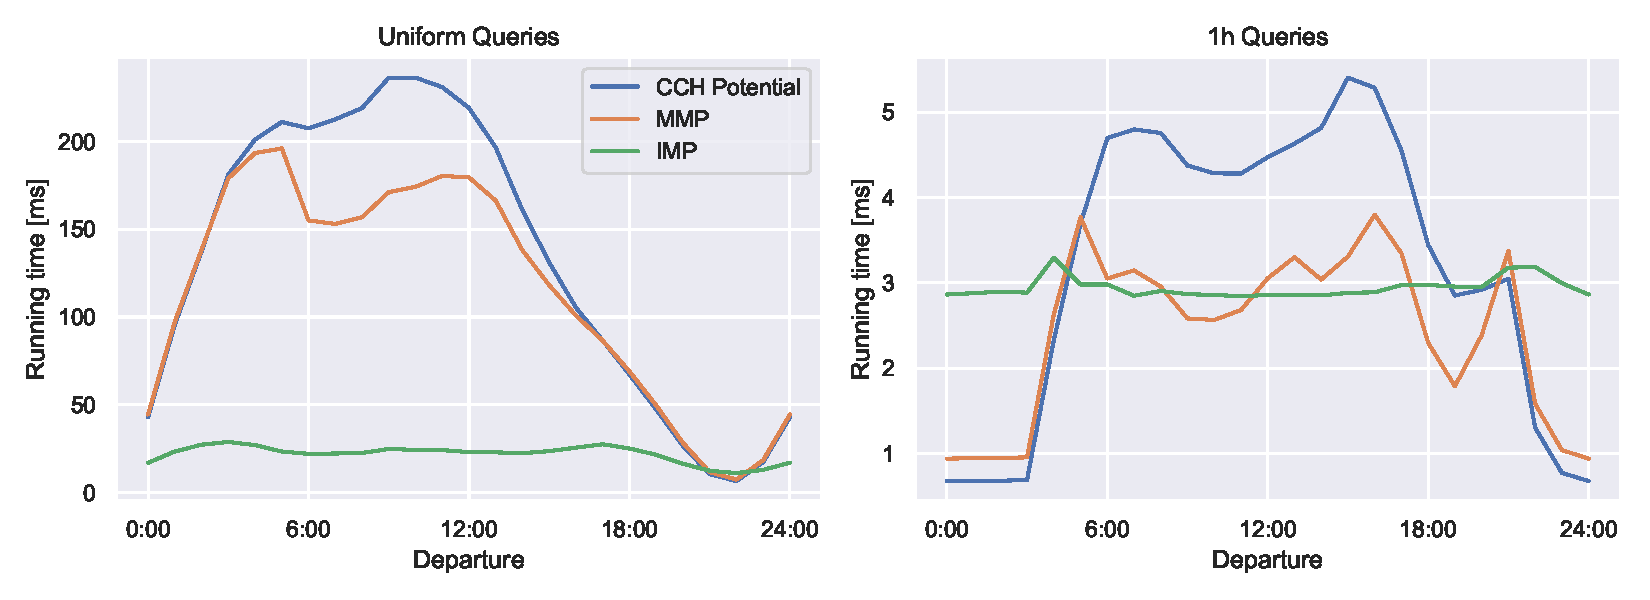
\includegraphics[width=\linewidth]{fig/perf_over_day.pdf}
\caption{
Average running time of 100\,K uniform and 1h queries on OSM Germany with only predicted traffic.
Each query has a departure drawn uniformly at random.
The resulting running times are grouped by the departure time hour.
}\label{fig:by_dep}
\end{figure}

Introducing live traffic decreases the quality of the potential estimates and thus increases search space sizes and running times.
For IMP this brings running times up to 38\,ms with heavy traffic which is still more than 90 times faster than Dijkstra's algorithm.
Surprisingly, for CCH-Potentials and MMP, heavier traffic seems to be easier to handle than lite traffic.
This is because we set the departures for the queries corresponding to the live traffic snapshot and use random departures for only predicted traffic.
However, the departure time has a significant influence on the performance.

Figure~\ref{fig:by_dep} depicts query performance by queried departure time over the course of the day.
Clearly, the departure time has a significant influence both for short-range and long-range queries.
For long-range queries, the peaks are shifted and somewhat smeared because of the time (on average four to five hours) covered in the query.
This dependence on the departure is the time why the heavy traffic (departure 15:41) appears to be easier than the lite (departure 10:21) for MMP and CCH-Potentials.
For IMP, the influence of the departure time is much smaller which makes it the fastest for all times on long-range queries.
For short-range queries, the other potentials are actually faster during the night due to the large overhead of the IMP.
Moreover, the MMP is roughly as fast as the IMP for 1h queries during the daytime.
Therefore, MMP may actually be a very simple and practical approach for many practical applications where short-range queries are much more prominent.

\begin{figure}
\centering
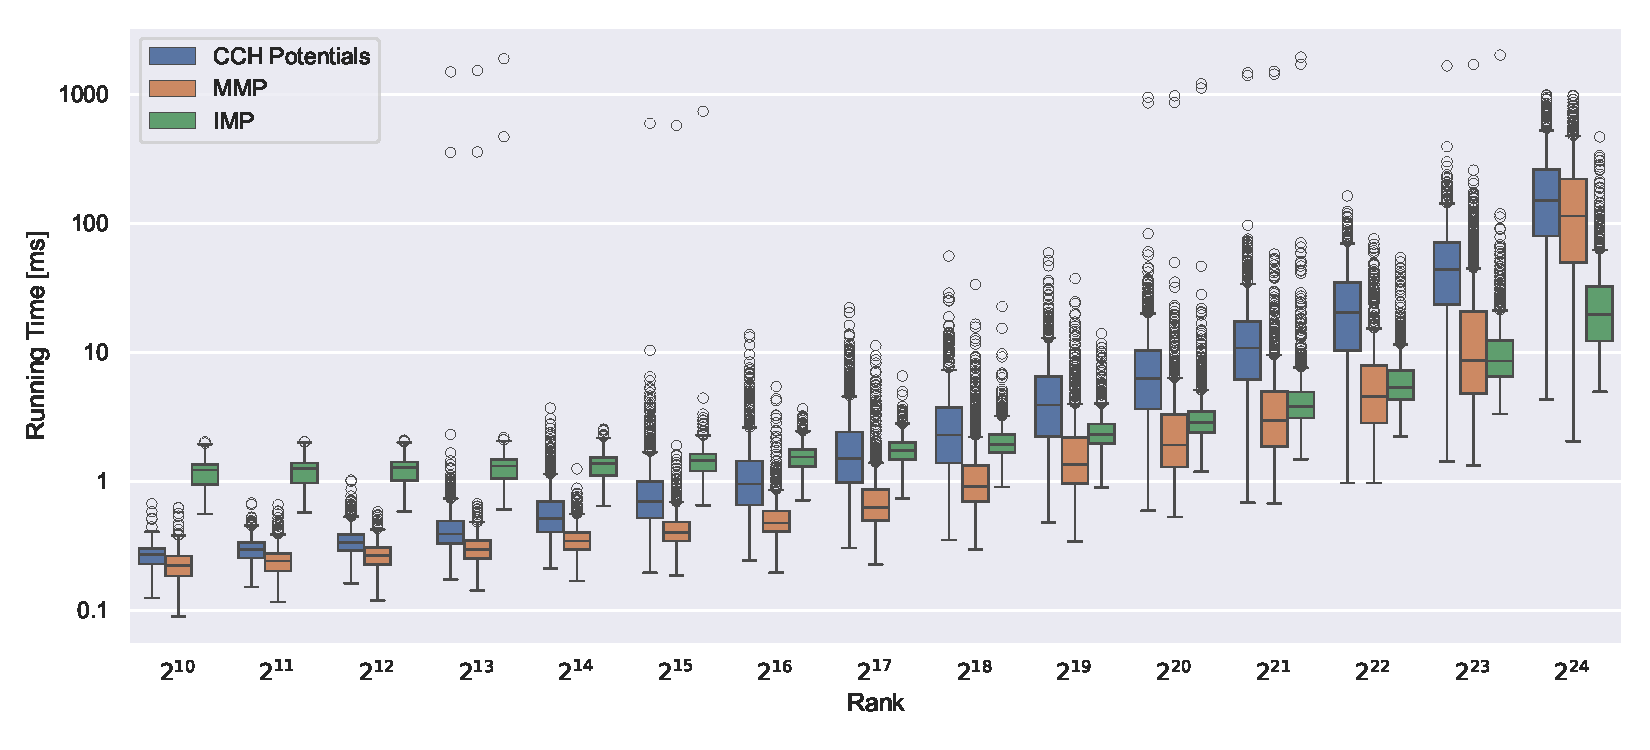
\includegraphics[width=\linewidth]{fig/ranks.pdf}
\caption{
Box plot of running times of 1000 queries per Dijkstra-rank on PTV Europe with live traffic and fixed departure at 07:47.
The boxes cover the range between the first and third quartile.
The band in the box indicates the median, the whiskers cover 1.5 times the interquartile range.
All other running times are indicated as outliers.
}\label{fig:ranks}
\end{figure}

In Figure~\ref{fig:ranks}, we investigate the performance by query distance.
The experiments confirms our analysis from the departure time experiment.
For short-range queries, IMP is slower than the other approaches because it is expensive to evaluate but it scales much better to long-range queries because of its tighter estimates.
Also the running times are much more stable and have a smaller variance.
Even for rank 24, most queries can be answered within a few tenths of milliseconds.
Nevertheless, the MMP is actually faster on most ranks.
Only at rank 24, the running times become as slow as the CCH-Potentials baseline.
The reason for the strong jump from 23 to 24 is that the mean query distance jumps from five to six hours on rank 23 to over eight hours which is longer than the longest covered interval.
Thus on rank 24, the MMP will fill back to a regular CCH-Potential on most queries.
We also observe a few strong outliers.
This happens because of blocked streets in the live traffic data.
When the target vertex of a query is only reachable through a blocked road segment, A* will traverse large parts of the networks until the blocked road opens up.
This affects all three potentials in the same way.

\begin{figure}
\centering
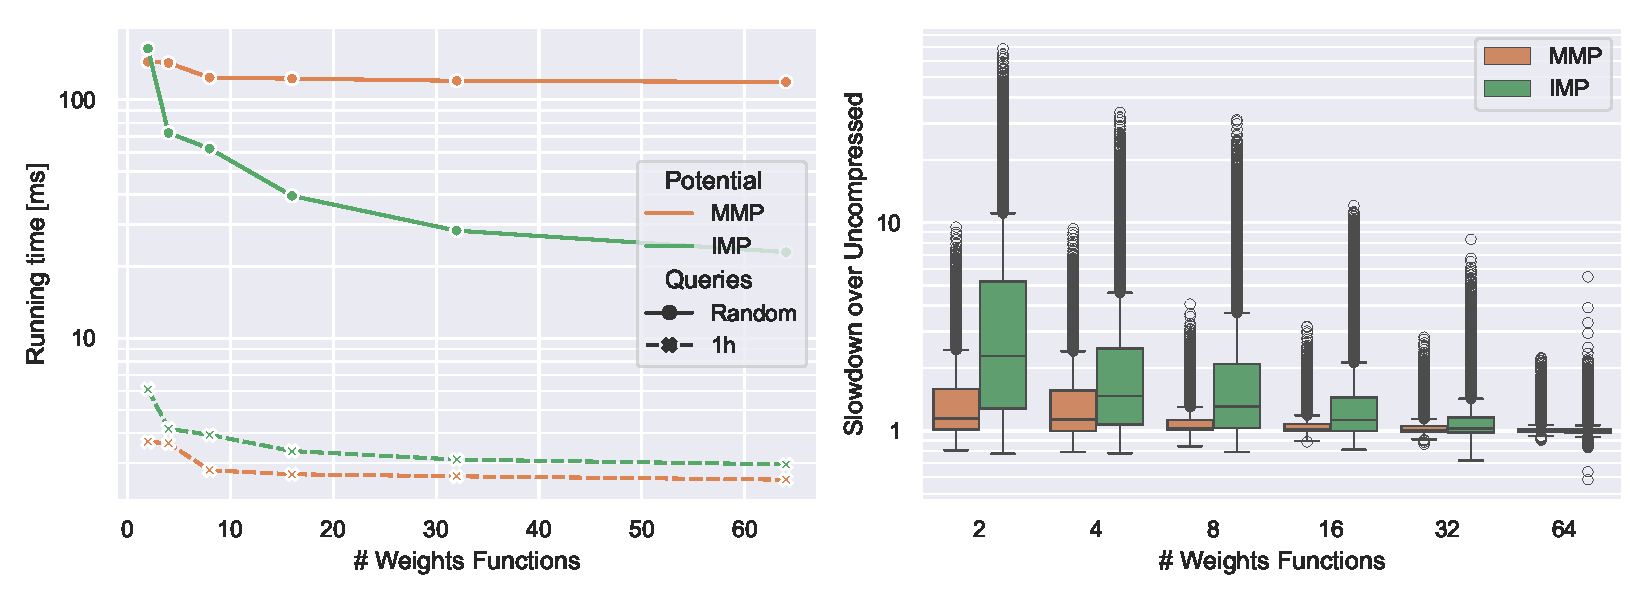
\includegraphics[width=\linewidth]{fig/compression.pdf}
\caption{
Mean running times of 100\,K queries on OSM Germany with only predicted traffic by number of remaining weight functions.
The second plot contains a boxplot of the per query relative slowdown over the running time of the respective query with all weight functions.
}\label{fig:compression}
\end{figure}

Finally, we investigate the effects of reducing the number of weight functions.
Figure~\ref{fig:compression} depicts the results.
The MMP appears to be very robust against compression.
We can reduce the number of weight functions to 16 (a memory usage reduction of about a factor of 6) before the slowdowns become noticeable in the mean running time.
However, the MMP also only achieves relatively small speed-ups compared to a CCH-Potential (rarely more than a factor of three).
Therefore, its robustness is not particularly surprising.
The IMP, which achieves much greater speed-ups is less robust against compression.
Nevertheless, we can reduce the memory consumption by a factor of about three (to 32 functions) and still achieve very decent query running times.
With 32 functions, the absolute memory consumption goes down to less than 20\,GB which is at least manageable.
% on long range queries still when reduced to 4 faster than MMP
The running time of the compression algorithm is generally relatively short compared to the rest of the preprocessing because of the efficient parallelization.
See Appendix~\ref{sec:appendix:parallelization} for further details.

\section{Conclusion}

In this paper, we proposed time-dependent A* potentials for efficient routing in time-dependent road networks with both predicted and live traffic.
We presented two realizations of time-dependent potentials with different trade-offs and showed how to apply them in this setting.
Both allow fast live traffic updates within a fraction of a minute.
We achieve query times two orders of magnitude faster than Dijkstra's algorithm and up to an order of magnitude faster than state-of-the-art time-independent potentials.
To the best of our knowledge, this makes our approach the first to achieve almost real-time query performance while allowing fast updates in this setting.

% \section{Typesetting instructions -- Summary}
% \label{sec:typesetting-summary}

% LIPIcs is a series of open access high-quality conference proceedings across all fields in informatics established in cooperation with Schloss Dagstuhl.
% In order to do justice to the high scientific quality of the conferences that publish their proceedings in the LIPIcs series, which is ensured by the thorough review process of the respective events, we believe that LIPIcs proceedings must have an attractive and consistent layout matching the standard of the series.
% Moreover, the quality of the metadata, the typesetting and the layout must also meet the requirements of other external parties such as indexing service, DOI registry, funding agencies, among others. The guidelines contained in this document serve as the baseline for the authors, editors, and the publisher to create documents that meet as many different requirements as possible.

% Please comply with the following instructions when preparing your article for a LIPIcs proceedings volume.
% \paragraph*{Minimum requirements}

% \begin{itemize}
% \item Use pdflatex and an up-to-date \LaTeX{} system.
% \item Use further \LaTeX{} packages and custom made macros carefully and only if required.
% \item Use the provided sectioning macros: \verb+\section+, \verb+\subsection+, \verb+\subsubsection+, \linebreak \verb+\paragraph+, \verb+\paragraph*+, and \verb+\subparagraph*+.
% \item Provide suitable graphics of at least 300dpi (preferably in PDF format).
% \item Use BibTeX and keep the standard style (\verb+plainurl+) for the bibliography.
% \item Please try to keep the warnings log as small as possible. Avoid overfull \verb+\hboxes+ and any kind of warnings/errors with the referenced BibTeX entries.
% \item Use a spellchecker to correct typos.
% \end{itemize}

% \paragraph*{Mandatory metadata macros}
% Please set the values of the metadata macros carefully since the information parsed from these macros will be passed to publication servers, catalogues and search engines.
% Avoid placing macros inside the metadata macros. The following metadata macros/environments are mandatory:
% \begin{itemize}
% \item \verb+\title+ and, in case of long titles, \verb+\titlerunning+.
% \item \verb+\author+, one for each author, even if two or more authors have the same affiliation.
% \item \verb+\authorrunning+ and \verb+\Copyright+ (concatenated author names)\\
% The \verb+\author+ macros and the \verb+\Copyright+ macro should contain full author names (especially with regard to the first name), while \verb+\authorrunning+ should contain abbreviated first names.
% \item \verb+\ccsdesc+ (ACM classification, see \url{https://www.acm.org/publications/class-2012}).
% \item \verb+\keywords+ (a comma-separated list of keywords).
% \item \verb+\relatedversion+ (if there is a related version, typically the ``full version''); please make sure to provide a persistent URL, e.\,g., at arXiv.
% \item \verb+\begin{abstract}...\end{abstract}+ .
% \end{itemize}

% \paragraph*{Please do not \ldots} %Do not override the \texttt{\seriesstyle}-defaults}
% Generally speaking, please do not override the \texttt{lipics-v2021}-style defaults. To be more specific, a short checklist also used by Dagstuhl Publishing during the final typesetting is given below.
% In case of \textbf{non-compliance} with these rules Dagstuhl Publishing will remove the corresponding parts of \LaTeX{} code and \textbf{replace it with the \texttt{lipics-v2021} defaults}. In serious cases, we may reject the LaTeX-source and expect the corresponding author to revise the relevant parts.
% \begin{itemize}
% \item Do not use a different main font. (For example, the \texttt{times} package is forbidden.)
% \item Do not alter the spacing of the \texttt{lipics-v2021.cls} style file.
% \item Do not use \verb+enumitem+ and \verb+paralist+. (The \texttt{enumerate} package is preloaded, so you can use
%  \verb+\begin{enumerate}[(a)]+ or the like.)
% \item Do not use ``self-made'' sectioning commands (e.\,g., \verb+\noindent{\bf My+ \verb+Paragraph}+).
% \item Do not hide large text blocks using comments or \verb+\iffalse+ $\ldots$ \verb+\fi+ constructions.
% \item Do not use conditional structures to include/exclude content. Instead, please provide only the content that should be published -- in one file -- and nothing else.
% \item Do not wrap figures and tables with text. In particular, the package \texttt{wrapfig} is not supported.
% \item Do not change the bibliography style. In particular, do not use author-year citations. (The
% \texttt{natbib} package is not supported.)
% \end{itemize}

% \enlargethispage{\baselineskip}

% This is only a summary containing the most relevant details. Please read the complete document ``LIPIcs: Instructions for Authors and the \texttt{lipics-v2021} Class'' for all details and don't hesitate to contact Dagstuhl Publishing (\url{mailto:publishing@dagstuhl.de}) in case of questions or comments:
% \href{http://drops.dagstuhl.de/styles/lipics-v2021/lipics-v2021-authors/lipics-v2021-authors-guidelines.pdf}{\texttt{http://drops.dagstuhl.de/styles/lipics-v2021/\newline lipics-v2021-authors/lipics-v2021-authors-guidelines.pdf}}

% \section{Lorem ipsum dolor sit amet}

% Lorem ipsum dolor sit amet, consectetur adipiscing elit \cite{DBLP:journals/cacm/Knuth74}. Praesent convallis orci arcu, eu mollis dolor. Aliquam eleifend suscipit lacinia. Maecenas quam mi, porta ut lacinia sed, convallis ac dui. Lorem ipsum dolor sit amet, consectetur adipiscing elit. Suspendisse potenti. Donec eget odio et magna ullamcorper vehicula ut vitae libero. Maecenas lectus nulla, auctor nec varius ac, ultricies et turpis. Pellentesque id ante erat. In hac habitasse platea dictumst. Curabitur a scelerisque odio. Pellentesque elit risus, posuere quis elementum at, pellentesque ut diam. Quisque aliquam libero id mi imperdiet quis convallis turpis eleifend.

% \begin{lemma}[Lorem ipsum]
% \label{lemma:lorem}
% Vestibulum sodales dolor et dui cursus iaculis. Nullam ullamcorper purus vel turpis lobortis eu tempus lorem semper. Proin facilisis gravida rutrum. Etiam sed sollicitudin lorem. Proin pellentesque risus at elit hendrerit pharetra. Integer at turpis varius libero rhoncus fermentum vitae vitae metus.
% \end{lemma}

% \begin{proof}
% Cras purus lorem, pulvinar et fermentum sagittis, suscipit quis magna.


% \proofsubparagraph*{Just some paragraph within the proof.}
% Nam liber tempor cum soluta nobis eleifend option congue nihil imperdiet doming id quod mazim placerat facer possim assum. Lorem ipsum dolor sit amet, consectetuer adipiscing elit, sed diam nonummy nibh euismod tincidunt ut laoreet dolore magna aliquam erat volutpat.
% \begin{claim}
% content...
% \end{claim}
% \begin{claimproof}
% content...
%     \begin{enumerate}
%         \item abc abc abc \claimqedhere{}
%     \end{enumerate}
% \end{claimproof}

% \end{proof}

% \begin{corollary}[Curabitur pulvinar, \cite{DBLP:books/mk/GrayR93}]
% \label{lemma:curabitur}
% Nam liber tempor cum soluta nobis eleifend option congue nihil imperdiet doming id quod mazim placerat facer possim assum. Lorem ipsum dolor sit amet, consectetuer adipiscing elit, sed diam nonummy nibh euismod tincidunt ut laoreet dolore magna aliquam erat volutpat.
% \end{corollary}

% \begin{proposition}\label{prop1}
% This is a proposition
% \end{proposition}

% \autoref{prop1} and \cref{prop1} \ldots

% \subsection{Curabitur dictum felis id sapien}

% Curabitur dictum \cref{lemma:curabitur} felis id sapien \autoref{lemma:curabitur} mollis ut venenatis tortor feugiat. Curabitur sed velit diam. Integer aliquam, nunc ac egestas lacinia, nibh est vehicula nibh, ac auctor velit tellus non arcu. Vestibulum lacinia ipsum vitae nisi ultrices eget gravida turpis laoreet. Duis rutrum dapibus ornare. Nulla vehicula vulputate iaculis. Proin a consequat neque. Donec ut rutrum urna. Morbi scelerisque turpis sed elit sagittis eu scelerisque quam condimentum. Pellentesque habitant morbi tristique senectus et netus et malesuada fames ac turpis egestas. Aenean nec faucibus leo. Cras ut nisl odio, non tincidunt lorem. Integer purus ligula, venenatis et convallis lacinia, scelerisque at erat. Fusce risus libero, convallis at fermentum in, dignissim sed sem. Ut dapibus orci vitae nisl viverra nec adipiscing tortor condimentum \cite{DBLP:journals/cacm/Dijkstra68a}. Donec non suscipit lorem. Nam sit amet enim vitae nisl accumsan pretium.

% \begin{lstlisting}[caption={Useless code.},label=list:8-6,captionpos=t,float,abovecaptionskip=-\medskipamount]
% for i:=maxint to 0 do
% begin
%     j:=square(root(i));
% end;
% \end{lstlisting}

% \subsection{Proin ac fermentum augue}

% Proin ac fermentum augue. Nullam bibendum enim sollicitudin tellus egestas lacinia euismod orci mollis. Nulla facilisi. Vivamus volutpat venenatis sapien, vitae feugiat arcu fringilla ac. Mauris sapien tortor, sagittis eget auctor at, vulputate pharetra magna. Sed congue, dui nec vulputate convallis, sem nunc adipiscing dui, vel venenatis mauris sem in dui. Praesent a pretium quam. Mauris non mauris sit amet eros rutrum aliquam id ut sapien. Nulla aliquet fringilla sagittis. Pellentesque eu metus posuere nunc tincidunt dignissim in tempor dolor. Nulla cursus aliquet enim. Cras sapien risus, accumsan eu cursus ut, commodo vel velit. Praesent aliquet consectetur ligula, vitae iaculis ligula interdum vel. Integer faucibus faucibus felis.

% \begin{itemize}
% \item Ut vitae diam augue.
% \item Integer lacus ante, pellentesque sed sollicitudin et, pulvinar adipiscing sem.
% \item Maecenas facilisis, leo quis tincidunt egestas, magna ipsum condimentum orci, vitae facilisis nibh turpis et elit.
% \end{itemize}

% \begin{remark}
% content...
% \end{remark}

% \section{Pellentesque quis tortor}

% Nec urna malesuada sollicitudin. Nulla facilisi. Vivamus aliquam tempus ligula eget ornare. Praesent eget magna ut turpis mattis cursus. Aliquam vel condimentum orci. Nunc congue, libero in gravida convallis \cite{DBLP:conf/focs/HopcroftPV75}, orci nibh sodales quam, id egestas felis mi nec nisi. Suspendisse tincidunt, est ac vestibulum posuere, justo odio bibendum urna, rutrum bibendum dolor sem nec tellus.

% \begin{lemma} [Quisque blandit tempus nunc]
% Sed interdum nisl pretium non. Mauris sodales consequat risus vel consectetur. Aliquam erat volutpat. Nunc sed sapien ligula. Proin faucibus sapien luctus nisl feugiat convallis faucibus elit cursus. Nunc vestibulum nunc ac massa pretium pharetra. Nulla facilisis turpis id augue venenatis blandit. Cum sociis natoque penatibus et magnis dis parturient montes, nascetur ridiculus mus.
% \end{lemma}

% Fusce eu leo nisi. Cras eget orci neque, eleifend dapibus felis. Duis et leo dui. Nam vulputate, velit et laoreet porttitor, quam arcu facilisis dui, sed malesuada risus massa sit amet neque.

% \section{Morbi eros magna}

% Morbi eros magna, vestibulum non posuere non, porta eu quam. Maecenas vitae orci risus, eget imperdiet mauris. Donec massa mauris, pellentesque vel lobortis eu, molestie ac turpis. Sed condimentum convallis dolor, a dignissim est ultrices eu. Donec consectetur volutpat eros, et ornare dui ultricies id. Vivamus eu augue eget dolor euismod ultrices et sit amet nisi. Vivamus malesuada leo ac leo ullamcorper tempor. Donec justo mi, tempor vitae aliquet non, faucibus eu lacus. Donec dictum gravida neque, non porta turpis imperdiet eget. Curabitur quis euismod ligula.


%%
%% Bibliography
%%

%% Please use bibtex, 

\bibliography{references}

\appendix

\section{Further Discussion of Traffic Model}\label{sec:appendix:model}

% TODO talk about -1 segment
% TODO visualize
% TODO inf

\section{Correctness Properties of Time-Dependent A* Potentials}\label{sec:appendix:correctness}

In this section, we analyze correctness properties for time-dependent A* potentials.
For the analysis, it is oftentimes more practical the use arrival time functions instead of travel time functions.
Given a travel time function $w$, we denote the respective arrival time function as $\hat{w}(uv, \tau) := w(uv, \tau) + \tau$.
With arrival time functions, we can represent path lengths simply as the composition of the edges arrival time functions.
Similarly to the time-independent case, we can define a modified weight function $w'$ such that running A* on a graph $G$ with time-dependent travel times $w$ with a time-dependent potential $\pi_t$ is equivalent to running Dijkstra's on the same graph with modified weights $w'$.
Consider a vertex $u$ with an arrival time of $\tau$.
In A*, its queue key is $\tau' = \hat{\pi}_t(u, \tau)$.
When relaxing an edge $uv$, we get a queue key of $\hat{\pi}_t(u, \hat{w}(uv, \tau))$ at $v$.
Thus, by definition we get $\hat{w}'(uv, \tau') = \hat{\pi}_t(v, \hat{w}(uv, \hat{\pi}_t(u)^{-1}(\tau')))$ where $\hat{\pi}_t(u)^{-1}$ is the inverted arrival time function, i.e.\ a \emph{departure time} function.
For $\hat{\pi}_t(u)^{-1}$ to be well defined, we need $\tau_1 \neq \tau_2 \implies \hat{\pi}_t(\tau_1) \neq \hat{\pi}_t(\tau_2)$.
Therefore, for potentials we require the \emph{strong First-In First-Out} property:
\[
\pi_t(v, \tau) < \pi_t(v, \tau + \epsilon) + \epsilon, v \in V, \tau \in T, \epsilon \geq 0
\]
Note that potentials which only adhere to the regular FIFO property in practice likely work just as well.
It just breaks the well-definedness of the modified weights for an theoretically equivalent run of Dijkstra's algorithm.

Shortest paths for these modified weights are the same es with the original weights.
Consider the weights of two different $s$-$t$ paths.
The initial potential at $s$ is the same for both paths, all the inner potential evaluations cancel out and the potentials at $s$ and the final potential evaluation at $t$ cannot change the order due to the FIFO property.

We can follow that when these modified weights do not have any negative travel times, then Dijkstra and thus A* will obtain correct result. % running time
This leads to the \emph{feasibility} property for time-dependent potentials:
\[
\hat{w}'(uv, \tau') = \hat{\pi}_t(v, \hat{w}(uv, \hat{\pi}_t(u)^{-1}(\tau'))) \geq \tau'
\]
To simplify correctness proofs for potentials, we reform this to a simpler equivalent property:
\begin{align*}
\hat{\pi}_t(v, \hat{w}(uv, \tau)) & \geq \hat{\pi}_t(u, \tau) \\
\pi_t(v, w(uv, \tau) + \tau) + w(uv, \tau) + \tau & \geq \pi_t(u, \tau) + \tau \\
\pi_t(v, w(uv, \tau) + \tau) + w(uv, \tau) - \pi_t(u, \tau) & \geq 0
\end{align*}
This formulation also shows that the time-dependent feasibility is a generalization to the classical feasibility property.

The third property is the \emph{lower bound} property:
\[
\pi_t(v, \tau) \leq \dist(v,t,\tau)
\]
With a potential fulfilling this property, A* will have found the shortest path once the target vertex was settled, even if the potential is not feasible.
This is because every shortest path vertex must have a queue key smaller than the target and by induction all these vertexes must have been settled before the target.
Also, even with negative travel times, negative cycles are not possible.
Consider a cycle $C$ starting and ending at vertex $v$.
The length of the cycle with the modified weights is $w'(C, \tau') = \hat{\pi}_t(v, \hat(w)(C, \hat{\pi}_t(u)^{-1}(\tau')))$ because all inner potential functions cancel out.
As $\hat{\pi}_t(v)$ has to adhere to the FIFO property, the length of $C$ cannot be negative.
Thus, A* with lower bound potentials will obtain correct results.
However, the running time may be exponential in the graph size.

Crucially, to guarantee correctness it is not necessary to adhere to these properties for all $\tau$.
Assume we are running A* to answer a query from $s$ to $t$ with departure $\tdep$.
Clearly, A* will never invoke the potential of vertex $v$ with $\tau < \dist(s,v,\tdep)$.
Therefore, it is sufficient to guarantee the strong FIFO property at vertex $v$ and the feasibility property for edge $vw$ for $\tau \geq \dist(s,v,\tdep)$.
For the lower bound property it even suffices to guarantee it only at exactly $\tau = \dist(s,v,\tdep)$.

\section{Optimizations}\label{sec:appendix:optimizations}

which we denote by $\dist^<(u,v)$

It has three steps.
In the first \emph{basic customization} step, each edge $uv \in E^+$ is processed such that $w^+(uv) = \dist^<(u,v)$.
This is already sufficient to apply the CH query algorithm and compute correct distances.
However, the augmented graph has more edges than necessary, which has a negative impact on query performance.
In the \emph{perfect customization}, edges $uv \in E^+$ are processed again to obtain a weight function $w^*(uv) = \dist(u,v)$.
The authors of~\cite{dsw-cch-15} proved that edges $uv$ where $w^+(uv) > w^*(uv)$ are not necessary to answer queries correctly.
Thus, in a final step, these edges are removed and a \emph{reduced augmented graph} $G^*=(V, E^*)$ is constructed.
All three customization steps can be parallelized efficiently~\cite{bsw-rttau-19}.

CATCHUp does not support a time-dependent \emph{perfect} customization.
However, a decent number of unnecessary edges can still be identified by running the time-independent perfect customization on $b^+_{\max}$ which yields $b^*_{\max}$.
Then, each edge $uv$ where $\dist_w(u,v,\tau) \leq b^*_{\max}(uv) < b^+_{\min}(uv) \leq \dist^<_w(u,v,\tau)$ can be removed.
% We will also utilize this insight for our time-dependent potentials.

\subparagraph{Multi-Metric-Potential.}
During the update phase, we also run the perfect customization for the upper bound and obtain $\comb^*_{\max}$.
This allows us to remove unnecessary edges and accelerate the query phase.
We remove edges $uv$ where $\dist^<_c(u,v) \geq l_{[0:00, 24:00]}^+(uv) > \comb^*_{\max}(uv) \geq \dist_c(u,v)$ for all weight functions.
We could remove even more edges if we were to check the condition for every lower bound weight function individually.
However, in this case we could not reuse the same reduced augmented graph topology for all weight functions.
As this would roughly double memory consumption we only remove edges which can be removed for all weight functions.
We parallelize the reduced graph constructions as described in~\cite{bsw-rttau-19}.
% % metric switching?

\subparagraph{Interval-Minimum-Potential.}
Similarly to the Multi-Metric Potential, we can identify unnecessary edges in the update phase and construct a smaller reduced augmented graph which accelerates queries.
Again we use the perfect customization to obtain $\comb^*_{\max}$ and remove edges $uv$ where $\comb^*_{\max}(uv) < b^+_{\min}(uv)$.% derive from sources when predicted upper bound valid again (this is the reason why not reduced in preprocessing)
% reduced graph bounds
% reduced graph buckets by predicted bounds
% bound switching
% evaluation time metric pruning

\section{Parallelization of Compression}\label{sec:appendix:parallelization}

% \section{Styles of lists, enumerations, and descriptions}\label{sec:itemStyles}

% List of different predefined enumeration styles:

% \begin{itemize}
% \item \verb|\begin{itemize}...\end{itemize}|
% \item \dots
% \item \dots
% %\item \dots
% \end{itemize}

% \begin{enumerate}
% \item \verb|\begin{enumerate}...\end{enumerate}|
% \item \dots
% \item \dots
% %\item \dots
% \end{enumerate}

% \begin{alphaenumerate}
% \item \verb|\begin{alphaenumerate}...\end{alphaenumerate}|
% \item \dots
% \item \dots
% %\item \dots
% \end{alphaenumerate}

% \begin{romanenumerate}
% \item \verb|\begin{romanenumerate}...\end{romanenumerate}|
% \item \dots
% \item \dots
% %\item \dots
% \end{romanenumerate}

% \begin{bracketenumerate}
% \item \verb|\begin{bracketenumerate}...\end{bracketenumerate}|
% \item \dots
% \item \dots
% %\item \dots
% \end{bracketenumerate}

% \begin{description}
% \item[Description 1] \verb|\begin{description} \item[Description 1]  ...\end{description}|
% \item[Description 2] Fusce eu leo nisi. Cras eget orci neque, eleifend dapibus felis. Duis et leo dui. Nam vulputate, velit et laoreet porttitor, quam arcu facilisis dui, sed malesuada risus massa sit amet neque.
% \item[Description 3]  \dots
% %\item \dots
% \end{description}

% \cref{testenv-proposition} and \autoref{testenv-proposition} ...

% \section{Theorem-like environments}\label{sec:theorem-environments}

% List of different predefined enumeration styles:

% \begin{theorem}\label{testenv-theorem}
% Fusce eu leo nisi. Cras eget orci neque, eleifend dapibus felis. Duis et leo dui. Nam vulputate, velit et laoreet porttitor, quam arcu facilisis dui, sed malesuada risus massa sit amet neque.
% \end{theorem}

% \begin{lemma}\label{testenv-lemma}
% Fusce eu leo nisi. Cras eget orci neque, eleifend dapibus felis. Duis et leo dui. Nam vulputate, velit et laoreet porttitor, quam arcu facilisis dui, sed malesuada risus massa sit amet neque.
% \end{lemma}

% \begin{corollary}\label{testenv-corollary}
% Fusce eu leo nisi. Cras eget orci neque, eleifend dapibus felis. Duis et leo dui. Nam vulputate, velit et laoreet porttitor, quam arcu facilisis dui, sed malesuada risus massa sit amet neque.
% \end{corollary}

% \begin{proposition}\label{testenv-proposition}
% Fusce eu leo nisi. Cras eget orci neque, eleifend dapibus felis. Duis et leo dui. Nam vulputate, velit et laoreet porttitor, quam arcu facilisis dui, sed malesuada risus massa sit amet neque.
% \end{proposition}

% \begin{conjecture}\label{testenv-conjecture}
% Fusce eu leo nisi. Cras eget orci neque, eleifend dapibus felis. Duis et leo dui. Nam vulputate, velit et laoreet porttitor, quam arcu facilisis dui, sed malesuada risus massa sit amet neque.
% \end{conjecture}

% \begin{observation}\label{testenv-observation}
% Fusce eu leo nisi. Cras eget orci neque, eleifend dapibus felis. Duis et leo dui. Nam vulputate, velit et laoreet porttitor, quam arcu facilisis dui, sed malesuada risus massa sit amet neque.
% \end{observation}

% \begin{exercise}\label{testenv-exercise}
% Fusce eu leo nisi. Cras eget orci neque, eleifend dapibus felis. Duis et leo dui. Nam vulputate, velit et laoreet porttitor, quam arcu facilisis dui, sed malesuada risus massa sit amet neque.
% \end{exercise}

% \begin{definition}\label{testenv-definition}
% Fusce eu leo nisi. Cras eget orci neque, eleifend dapibus felis. Duis et leo dui. Nam vulputate, velit et laoreet porttitor, quam arcu facilisis dui, sed malesuada risus massa sit amet neque.
% \end{definition}

% \begin{example}\label{testenv-example}
% Fusce eu leo nisi. Cras eget orci neque, eleifend dapibus felis. Duis et leo dui. Nam vulputate, velit et laoreet porttitor, quam arcu facilisis dui, sed malesuada risus massa sit amet neque.
% \end{example}

% \begin{note}\label{testenv-note}
% Fusce eu leo nisi. Cras eget orci neque, eleifend dapibus felis. Duis et leo dui. Nam vulputate, velit et laoreet porttitor, quam arcu facilisis dui, sed malesuada risus massa sit amet neque.
% \end{note}

% \begin{note*}
% Fusce eu leo nisi. Cras eget orci neque, eleifend dapibus felis. Duis et leo dui. Nam vulputate, velit et laoreet porttitor, quam arcu facilisis dui, sed malesuada risus massa sit amet neque.
% \end{note*}

% \begin{remark}\label{testenv-remark}
% Fusce eu leo nisi. Cras eget orci neque, eleifend dapibus felis. Duis et leo dui. Nam vulputate, velit et laoreet porttitor, quam arcu facilisis dui, sed malesuada risus massa sit amet neque.
% \end{remark}

% \begin{remark*}
% Fusce eu leo nisi. Cras eget orci neque, eleifend dapibus felis. Duis et leo dui. Nam vulputate, velit et laoreet porttitor, quam arcu facilisis dui, sed malesuada risus massa sit amet neque.
% \end{remark*}

% \begin{claim}\label{testenv-claim}
% Fusce eu leo nisi. Cras eget orci neque, eleifend dapibus felis. Duis et leo dui. Nam vulputate, velit et laoreet porttitor, quam arcu facilisis dui, sed malesuada risus massa sit amet neque.
% \end{claim}

% \begin{claim*}\label{testenv-claim2}
% Fusce eu leo nisi. Cras eget orci neque, eleifend dapibus felis. Duis et leo dui. Nam vulputate, velit et laoreet porttitor, quam arcu facilisis dui, sed malesuada risus massa sit amet neque.
% \end{claim*}

% \begin{proof}
% Fusce eu leo nisi. Cras eget orci neque, eleifend dapibus felis. Duis et leo dui. Nam vulputate, velit et laoreet porttitor, quam arcu facilisis dui, sed malesuada risus massa sit amet neque.
% \end{proof}

% \begin{claimproof}
% Fusce eu leo nisi. Cras eget orci neque, eleifend dapibus felis. Duis et leo dui. Nam vulputate, velit et laoreet porttitor, quam arcu facilisis dui, sed malesuada risus massa sit amet neque.
% \end{claimproof}

\end{document}
